\documentclass{acm_proc_article-sp}

\usepackage{url}

\begin{document}

\title{CUTE: C++ Unit Testing Easier}

\numberofauthors{2}

\author{
% 1st. author
\alignauthor
Peter Sommerlad\\
       \affaddr{Institute for Software}\\
       \affaddr{Oberseestrasse 10}\\
       \affaddr{8640 Rapperswil}\\
       \email{peter.sommerlad@hsr.ch}
% 2nd. author
\alignauthor
Emanuel Graf\\
       \affaddr{Institute for Software}\\
       \affaddr{Oberseestrasse 10}\\
       \affaddr{8640 Rapperswil}\\
       \email{emanuel.graf@hsr.ch}
}


\maketitle
\begin{abstract}
This article describes the design and use of the CUTE C++ testing framework and its integration into the 
Eclipse C++ Development Tooling.

Unit testing supports code quality and is a corner stone of agile software development. CUTE and its 
Eclipse plug-in are an easy to use C++ testing framework.

\end{abstract}



\keywords{Unit Testing, C++, Eclipse}

\section{Introduction}
Automated unit testing supports high quality of program code, even under inevitable change and 
refactoring. As a side effect, unit tested code often has a better structure. Java developers are 
used to unit testing because of JUnit and its tight integration into IDEs like Eclipse. C++ programmers 
lacked the tool support for easy-to-use unit testing, even though the language's complexity asks for it. 
Refactoring and simplifying C++ code without tests is very hard and error-prone.

\section{Using CUTE}
Writing a unit test using CUTE is simple. A test is a simple parameterless void function there is no 
need to inherit from a test class.
\begin{verbatim}
#include "cute.h"
int theAnswer = 42;

void mysimpletest(){
  ASSERT(theAnswer == 6*7);
}
\end{verbatim}
In addition each test has a name, so that it can be easier identified. That name is either given during 
construction using the CUTE() macro or derived from the function's typeid.

Running a single test is not very usefull. But having a larger collection of test cases and 
running them  after every check in on a build server, is what makes unit testing so powerful. So there is 
a need for running many tests at once.

CUTE don't uses the Composite Design Pattern \cite{DesignPatterns} for implementing the container for 
these test cases. Instead test suites in CUTE are vectors containing a sequence of test cases. Thus we 
can avoid the strong coupling caused by inheritance and the lower cohesion in the container class, because 
the container don't need to support the composite interface. Test cases can be added to the suite using 
the \verb|push_back()| method inherited from vector or the overloaded \verb|+=| operator.

Since C++ lack some of the reflection mechanisms available in Java, we have to write our own main 
function for testing. For simple cases we only instantiate a runner object and pass our test for 
running it. Reporting the test results is so common, that CUTE provides a means to configure the runner 
with a listener passed as template parameter.

\begin{verbatim}
void runSuite(){
  cute::suite s;
  s.push_back(CUTE(mysimpletest));
  cute::ide_listener lis;
  cute::makeRunner(lis)(s, "The Suite");
}

int main(){
  runSuite();
}
\end{verbatim}

\section{Eclipse CDT Integration}
A good integration into a development environment simplifies the use of a testing framework. Additionally 
a good integration can improve the developers acceptance to write tests, so writing unit tests becomes 
a natural part of writing source code.

The CUTE Eclipse Plug-in\footnote{Update Site: \url{http://ifs.hsr.ch/cute/updatesite/}} integrates the 
CUTE testing framework into the Eclipse C/C++ Development Tooling (CDT)
\footnote{\url{http://www.eclipse.org/cdt/}} similar to the JUnit integration for the Eclipse Java 
Development Tools\footnote{\url{http://www.eclipse.org/jdt/}}. The plug-in's project creation wizards 
supports the developer by setting up a project including the necessary CUTE headers and the corresponding 
compiler and linker settings. A specialized wizard exists to create a test project for an already 
existing library project.

The plug-in uses the standard cute runner with a special output listener that writes the test results to 
\verb|std::cout| using a defined format. This output is parsed and an internal model of the test and there 
result is build. The results of the tests are presented to the developer by the result view. Therefore the 
result view can be used with other test frameworks as long as they provied the same output as the 
\verb|cute::eclipse_listener|.

CUTE's result view provides all the important features Java developer know from the JUnit-plug-in:
\begin{itemize}
 \item Red / Green Bar
 \item test navigator
 \item diff-viewer for failing tests
\end{itemize}

\begin{figure}
 \centering
 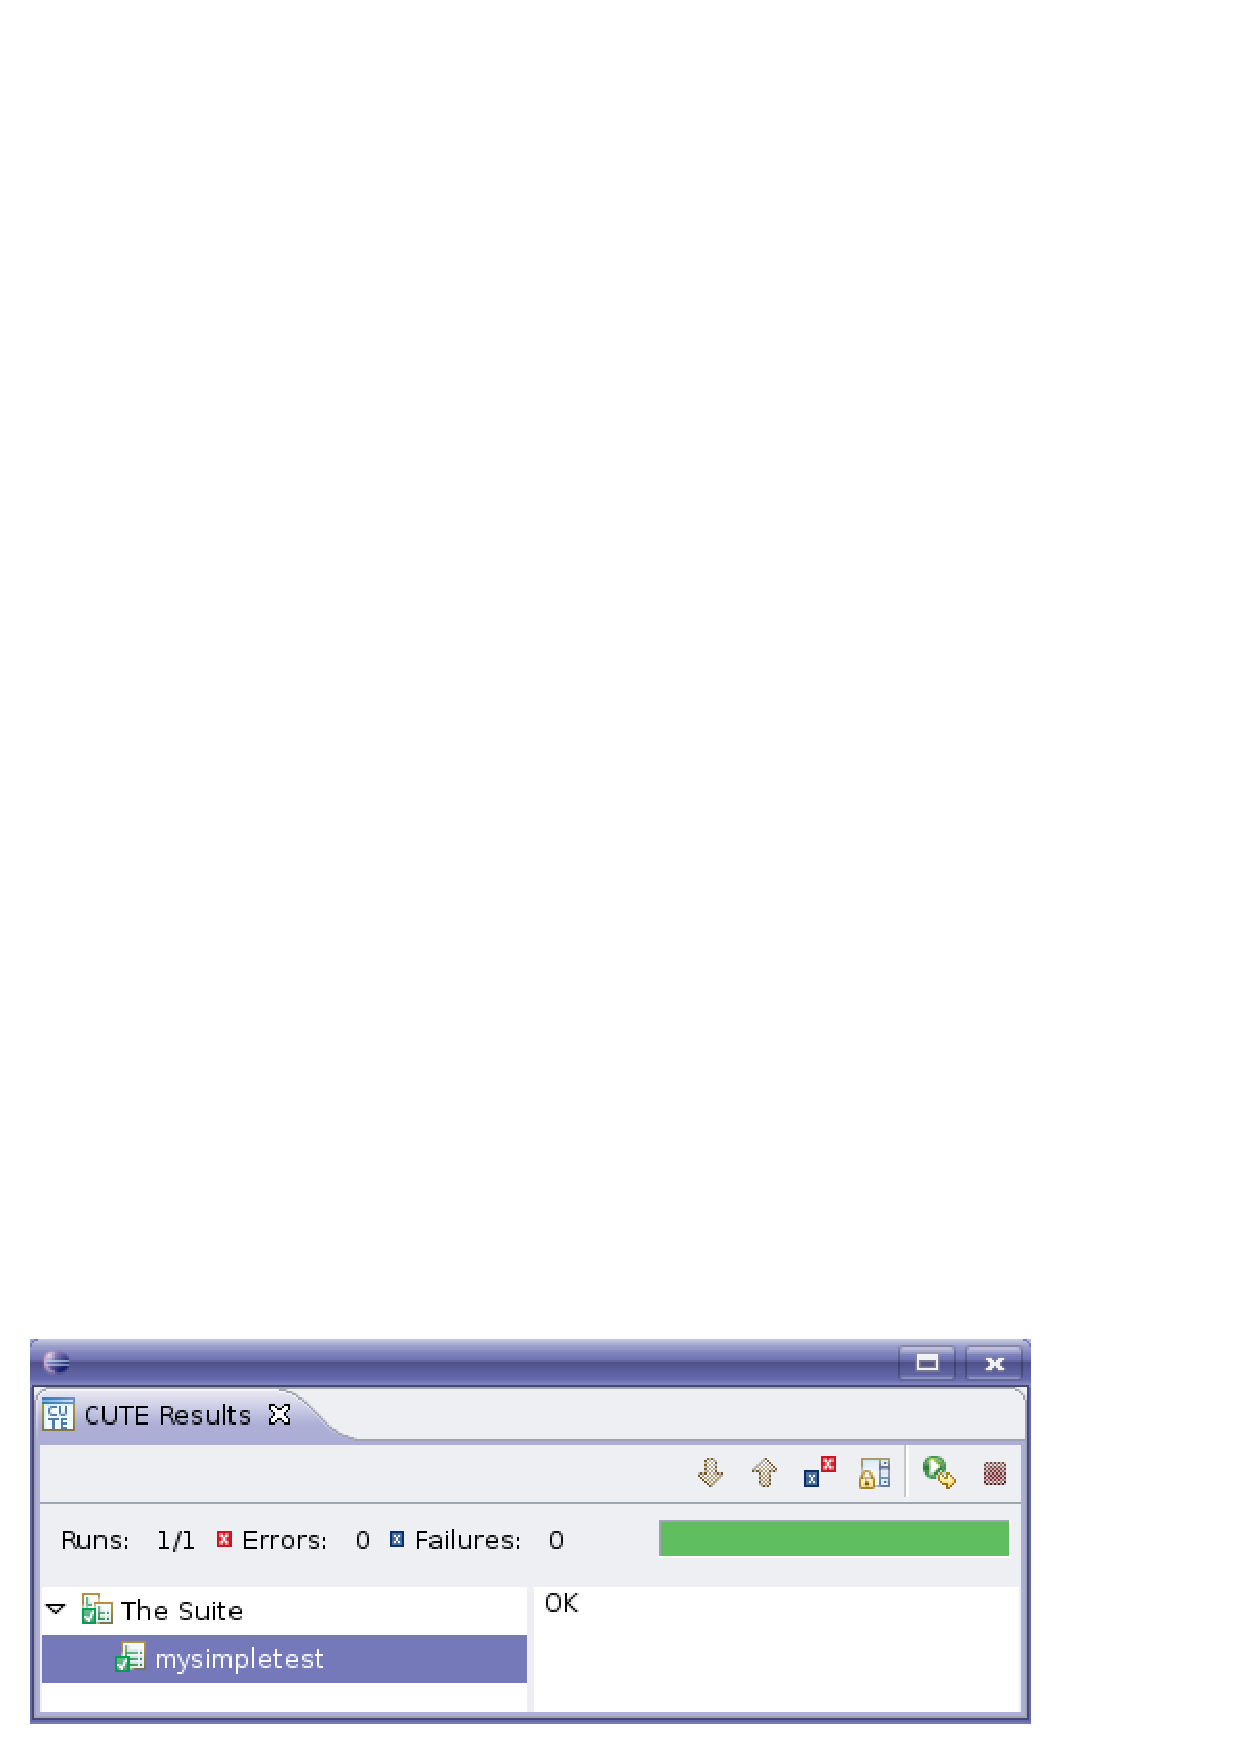
\includegraphics[width=0.48\textwidth]{results.png}
 \caption{\label{result View}CUTE result view}
\end{figure}

\section{Requirements and Outlook}
CUTE needs \verb|boost::bind| and \verb|boost::function| from the Boost\footnote{\url{http://www.boost.org/}} 
library that are part of the proposed C++ standard extension \verb|std::tr1|.

There are many ideas for extending CUTE to make it a more convenient environment to live in. 
For example, better integration into other IDEs like Visual Studio.

\bibliographystyle{abbrv}
%\bibliography{sigproc}  % sigproc.bib is the name of the Bibliography in this
\bibliography{bibliography}

\balancecolumns
% That's all folks!
\end{document}
